\documentclass[11pt]{amsbook}
\usepackage[turkish]{babel}

\usepackage{../Ceyhun}	
\usepackage{../amsTurkish}

\usepackage{graphicx}
\usepackage{lipsum}



\begin{document}
\hPage{103}
\begin{figure}[htb]
	\centering
	

	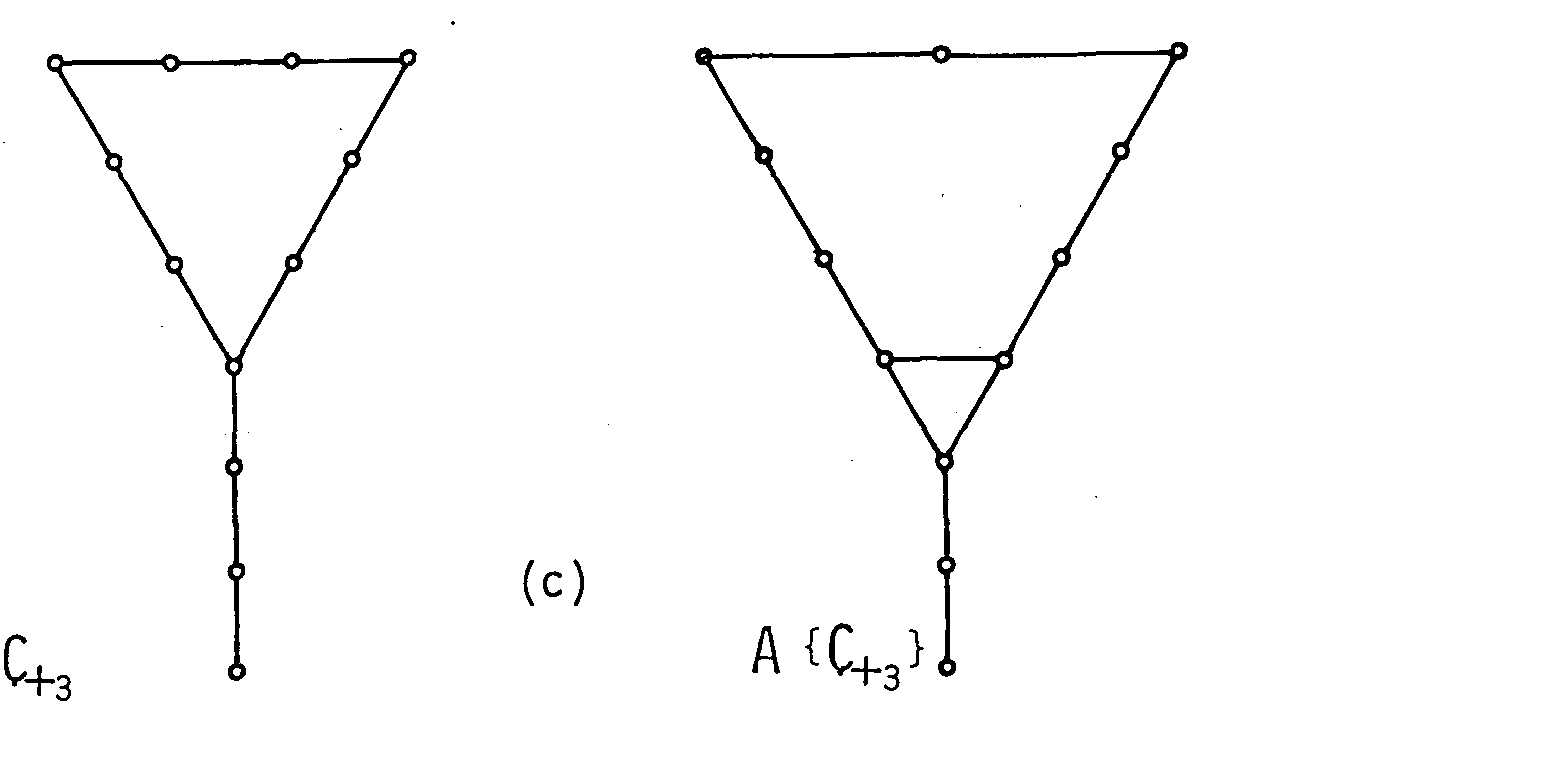
\includegraphics[keepaspectratio=true,scale=0.4]{images/ceyhun-103-fig01}
	\caption{Ayrıt ve katkılı ayrıt çizgilerine örnekler.}
\end{figure}
\\
Euler ya da Hamilton çizgesi olma özelliğinin,\\
ayrıt ve katkılı ayrıt çizgeleri üzerinde nasıl\\
etkilendiğine değgin aşağıdaki teoremleri\\
tanıtlamadan vereceğiz.\\
\begin{theorem}
Eğer $Ç$ Euler çizgesi ise, $A \{Ç\}$\\
hem Euler hem de Hamilton\\
çizgesidir.\\
\end{theorem}
\begin{theorem}
Eğer $Ç$ Hamilton çizgesi ise,\\
$A\{Ç\}$ de Hamilton cizgesidir.\\
\end{theorem}

Bu teormelerein terslerinin doğru olmadığı gözden\\
kaçmamalıdır. Başka bir deyişle,$A\{Ç\}$ nin hem\\
Euler hem de Hamilton çizgesi olması,$\{Ç\}$ nin Euler\\
çizgesi olacağı anlamına gelmez. Örneğin,\\



\end{document}